\documentclass[]{article}
\usepackage{lmodern}
\usepackage{amssymb,amsmath}
\usepackage{ifxetex,ifluatex}
\usepackage{fixltx2e} % provides \textsubscript
\ifnum 0\ifxetex 1\fi\ifluatex 1\fi=0 % if pdftex
  \usepackage[T1]{fontenc}
  \usepackage[utf8]{inputenc}
\else % if luatex or xelatex
  \ifxetex
    \usepackage{mathspec}
  \else
    \usepackage{fontspec}
  \fi
  \defaultfontfeatures{Ligatures=TeX,Scale=MatchLowercase}
\fi
% use upquote if available, for straight quotes in verbatim environments
\IfFileExists{upquote.sty}{\usepackage{upquote}}{}
% use microtype if available
\IfFileExists{microtype.sty}{%
\usepackage{microtype}
\UseMicrotypeSet[protrusion]{basicmath} % disable protrusion for tt fonts
}{}
\usepackage[margin=1in]{geometry}
\usepackage{hyperref}
\hypersetup{unicode=true,
            pdftitle={Visuals Portfolio},
            pdfauthor={Ashley Bleggi},
            pdfborder={0 0 0},
            breaklinks=true}
\urlstyle{same}  % don't use monospace font for urls
\usepackage{longtable,booktabs}
\usepackage{graphicx,grffile}
\makeatletter
\def\maxwidth{\ifdim\Gin@nat@width>\linewidth\linewidth\else\Gin@nat@width\fi}
\def\maxheight{\ifdim\Gin@nat@height>\textheight\textheight\else\Gin@nat@height\fi}
\makeatother
% Scale images if necessary, so that they will not overflow the page
% margins by default, and it is still possible to overwrite the defaults
% using explicit options in \includegraphics[width, height, ...]{}
\setkeys{Gin}{width=\maxwidth,height=\maxheight,keepaspectratio}
\IfFileExists{parskip.sty}{%
\usepackage{parskip}
}{% else
\setlength{\parindent}{0pt}
\setlength{\parskip}{6pt plus 2pt minus 1pt}
}
\setlength{\emergencystretch}{3em}  % prevent overfull lines
\providecommand{\tightlist}{%
  \setlength{\itemsep}{0pt}\setlength{\parskip}{0pt}}
\setcounter{secnumdepth}{5}
% Redefines (sub)paragraphs to behave more like sections
\ifx\paragraph\undefined\else
\let\oldparagraph\paragraph
\renewcommand{\paragraph}[1]{\oldparagraph{#1}\mbox{}}
\fi
\ifx\subparagraph\undefined\else
\let\oldsubparagraph\subparagraph
\renewcommand{\subparagraph}[1]{\oldsubparagraph{#1}\mbox{}}
\fi

%%% Use protect on footnotes to avoid problems with footnotes in titles
\let\rmarkdownfootnote\footnote%
\def\footnote{\protect\rmarkdownfootnote}

%%% Change title format to be more compact
\usepackage{titling}

% Create subtitle command for use in maketitle
\newcommand{\subtitle}[1]{
  \posttitle{
    \begin{center}\large#1\end{center}
    }
}

\setlength{\droptitle}{-2em}

  \title{Visuals Portfolio}
    \pretitle{\vspace{\droptitle}\centering\huge}
  \posttitle{\par}
  \subtitle{Last Updated May 24, 2018}
  \author{Ashley Bleggi}
    \preauthor{\centering\large\emph}
  \postauthor{\par}
    \date{}
    \predate{}\postdate{}
  

\begin{document}
\maketitle

{
\setcounter{tocdepth}{4}
\tableofcontents
}
\section{Stronger by Science}\label{stronger-by-science}

\textbf{Context:}\\
The visuals below were produced from monthly survey data following
strength-training athletes. The goal of this study is to conduct
Survival Analysis on strength athletes, specifically ``powerlifters,''
and identify any significant trends in injury reporting.

\begin{longtable}[]{@{}ll@{}}
\toprule
\begin{minipage}[b]{0.16\columnwidth}\raggedright\strut
Variable\strut
\end{minipage} & \begin{minipage}[b]{0.78\columnwidth}\raggedright\strut
Definition\strut
\end{minipage}\tabularnewline
\midrule
\endhead
\begin{minipage}[t]{0.16\columnwidth}\raggedright\strut
Uninjured\strut
\end{minipage} & \begin{minipage}[t]{0.78\columnwidth}\raggedright\strut
Subjects who have not yet reported an injury. They will continue
receiving surveys until the end of the research period or until they
sustain an injury.\strut
\end{minipage}\tabularnewline
\begin{minipage}[t]{0.16\columnwidth}\raggedright\strut
\strut
\end{minipage}\tabularnewline
\begin{minipage}[t]{0.16\columnwidth}\raggedright\strut
Injured\strut
\end{minipage} & \begin{minipage}[t]{0.78\columnwidth}\raggedright\strut
Subjects who have reported sustaining an injury in the last 30 days of
receiving that month's survey. These subjects will stop receiving
surveys from that point on.\strut
\end{minipage}\tabularnewline
\begin{minipage}[t]{0.16\columnwidth}\raggedright\strut
\strut
\end{minipage}\tabularnewline
\begin{minipage}[t]{0.16\columnwidth}\raggedright\strut
Lost to Followup\strut
\end{minipage} & \begin{minipage}[t]{0.78\columnwidth}\raggedright\strut
Subjects who had not reported having an injury, but stopped responding
to surveys.\strut
\end{minipage}\tabularnewline
\begin{minipage}[t]{0.16\columnwidth}\raggedright\strut
\strut
\end{minipage}\tabularnewline
\begin{minipage}[t]{0.16\columnwidth}\raggedright\strut
Type\strut
\end{minipage} & \begin{minipage}[t]{0.78\columnwidth}\raggedright\strut
General ``type'' or location of injuries reported by subjects.\strut
\end{minipage}\tabularnewline
\bottomrule
\end{longtable}

\subsection{Faceted Stacked Bar Chart}\label{faceted-stacked-bar-chart}

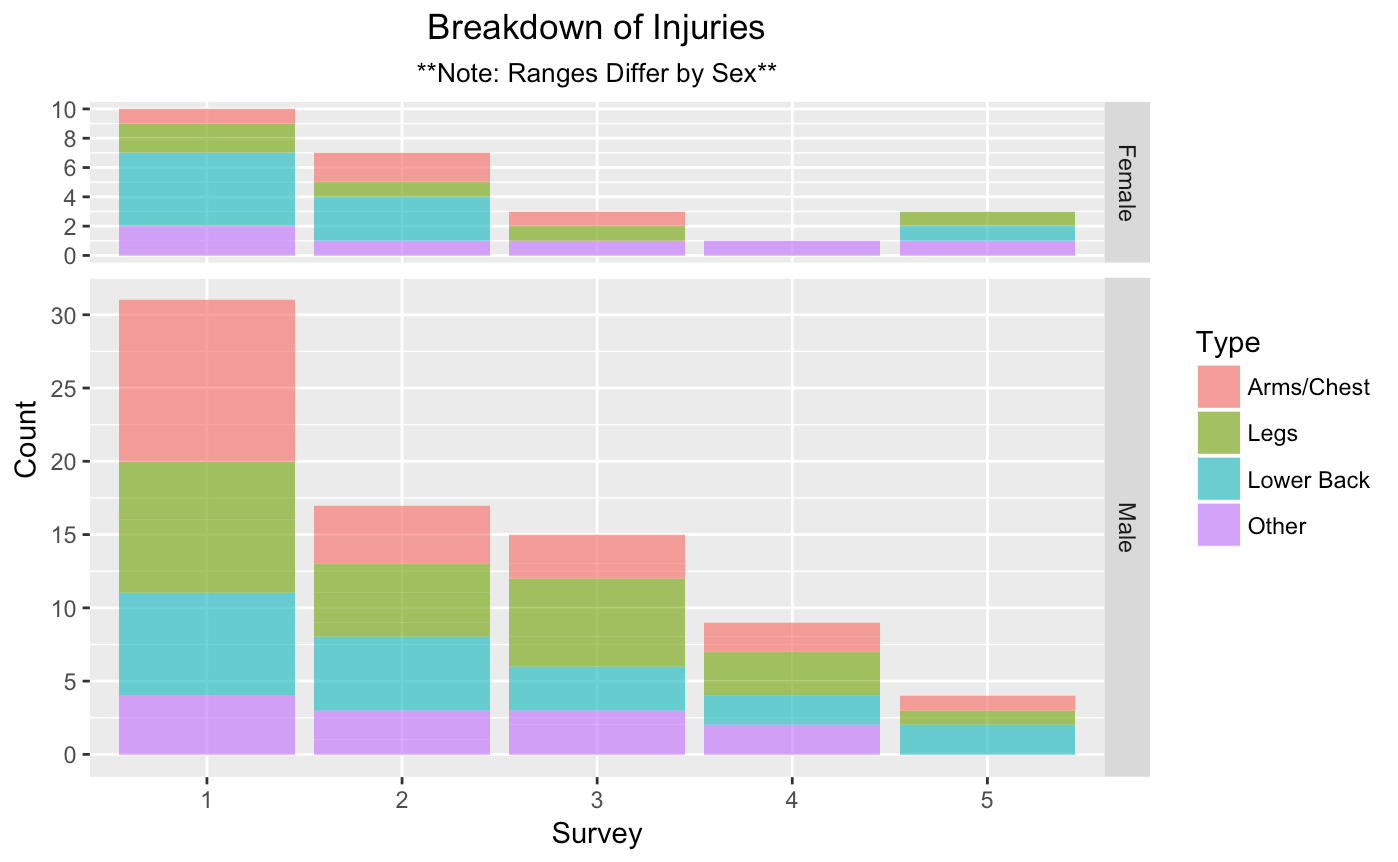
\includegraphics[width=1\linewidth]{images/BreakdownInjuries} The above
visual shows the change in the proportion of injury types by survey,
separated by the sex of respondents.

\subsection{Side-by-side Bar Chart}\label{side-by-side-bar-chart}

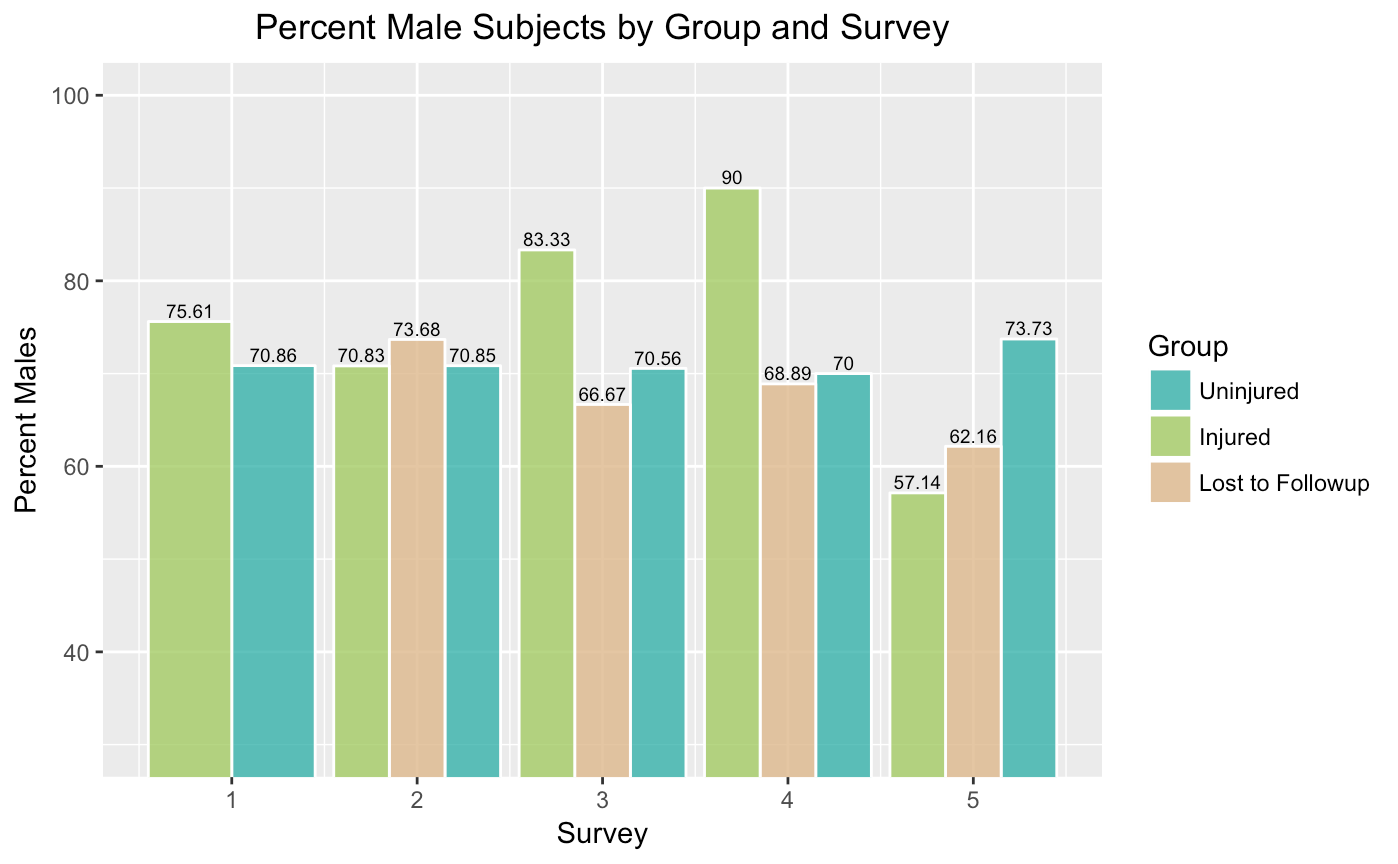
\includegraphics[width=1\linewidth]{images/PercentMaleSubjects} The
above visual shows change in the the proportion of male respondents by
survey and group.

\subsection{Layered \& Faceted Density
Plots}\label{layered-faceted-density-plots}

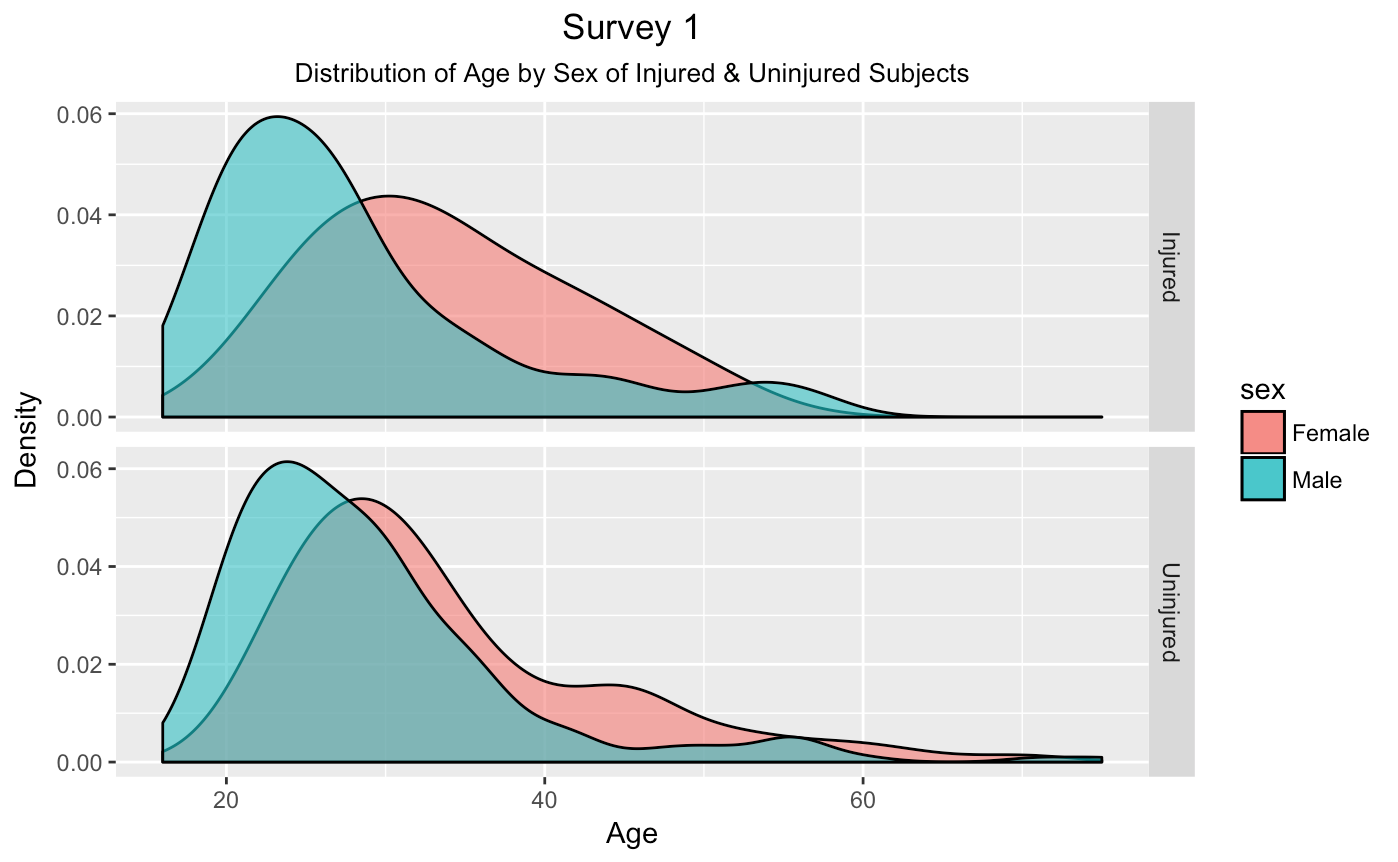
\includegraphics[width=1\linewidth]{images/DistAgeSex1} This visual
shows the baseline distribution of Age and Sex of the subjects who
responded to the first survey.

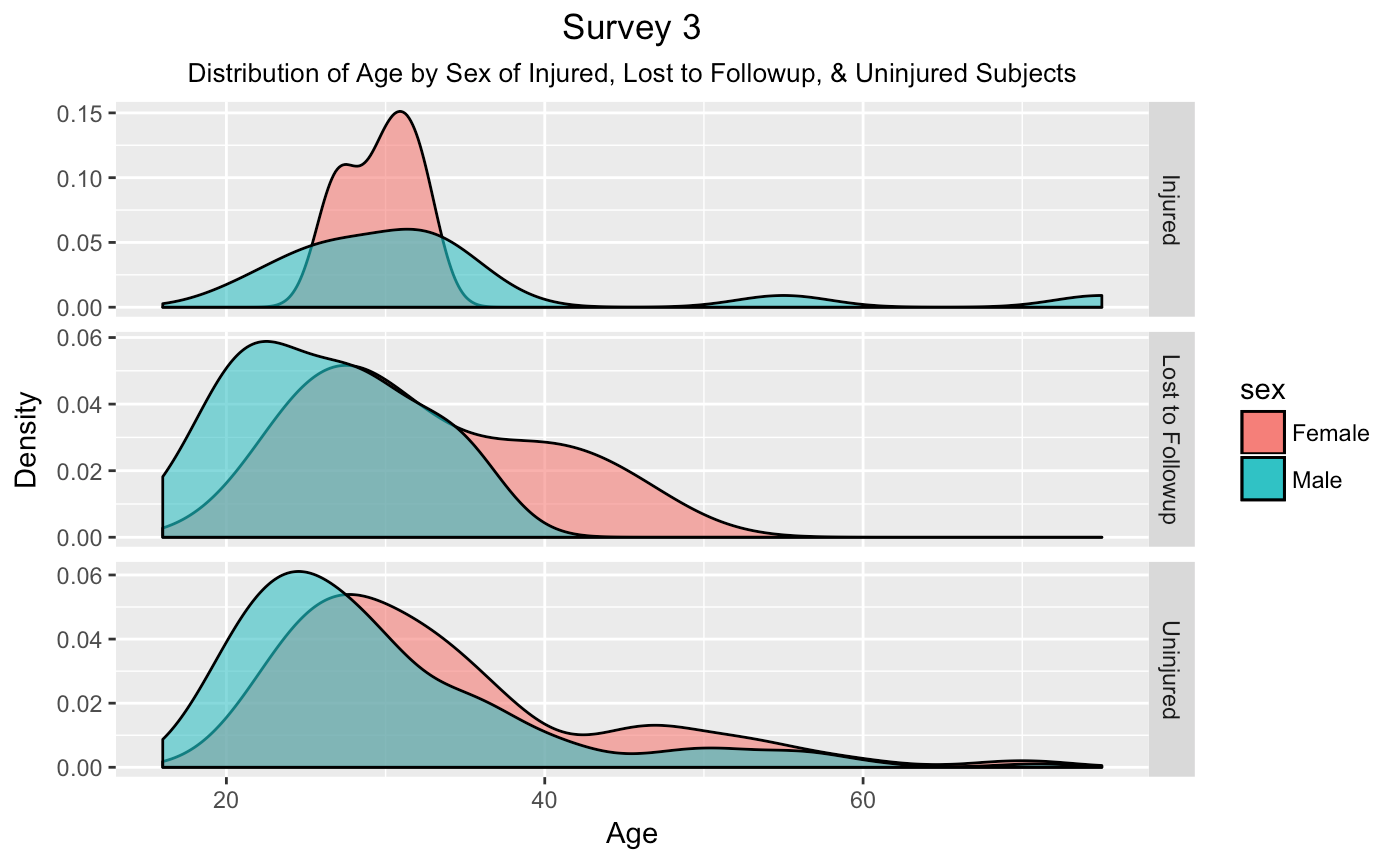
\includegraphics[width=1\linewidth]{images/DistAgeSex3} This visuals
shows how the age distribution changed by the third survey responses,
the groups now including those who stopped responding after the second
survey. The uninjured group remains nearly identical.

\section{Fifa Soccer Analysis}\label{fifa-soccer-analysis}

\textbf{Context:}\\
The goal of this project was to determine what skills (Attributes) are
most closely associated with what makes a ``good'' attacking soccer
player in the popular FIFA soccer game. My team and I pulled a data set
of the most recent FIFA game from kaggle.com
(\url{https://www.kaggle.com/thec03u5/fifa-18-demo-player-dataset}) for
use in a final project. Below are two of the final deliverables. We
sought to find what attributes correlate most closely with high scoring
players in the forward, wing, and striker positions.

\subsection{Correlation Plot}\label{correlation-plot}

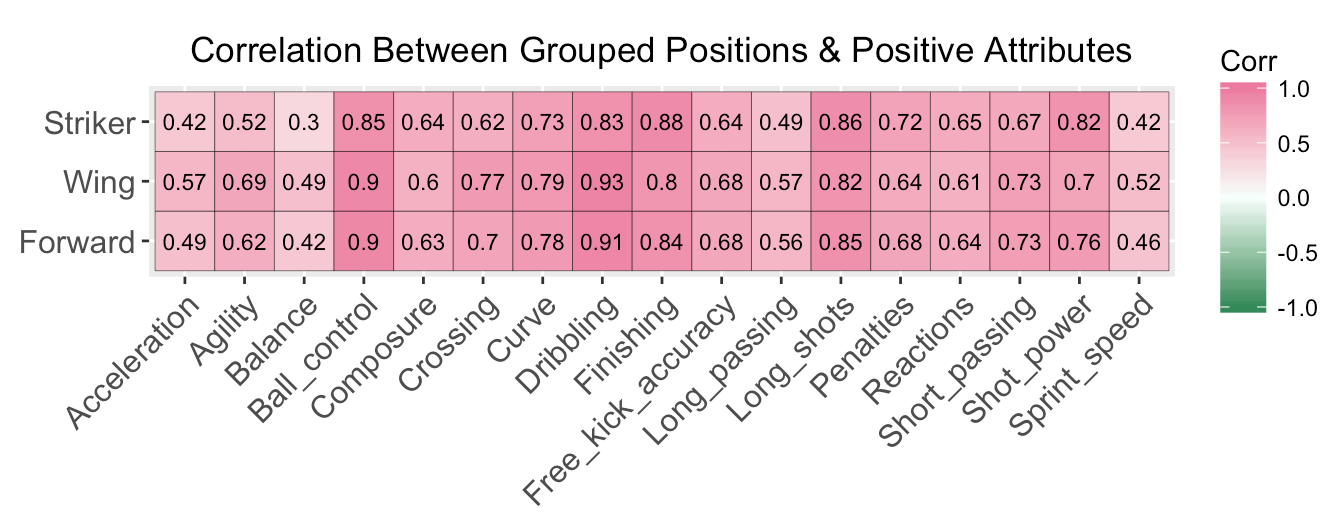
\includegraphics[width=1\linewidth]{images/corrplot1} The above visual
shows all the attributes that had a positive correlation with high
scoring players in Striker, Wing, and Forward player positions.
Previously, all the negative and 0 correlations were filtered out.

\subsection{Scatter-Correlation Plot}\label{scatter-correlation-plot}

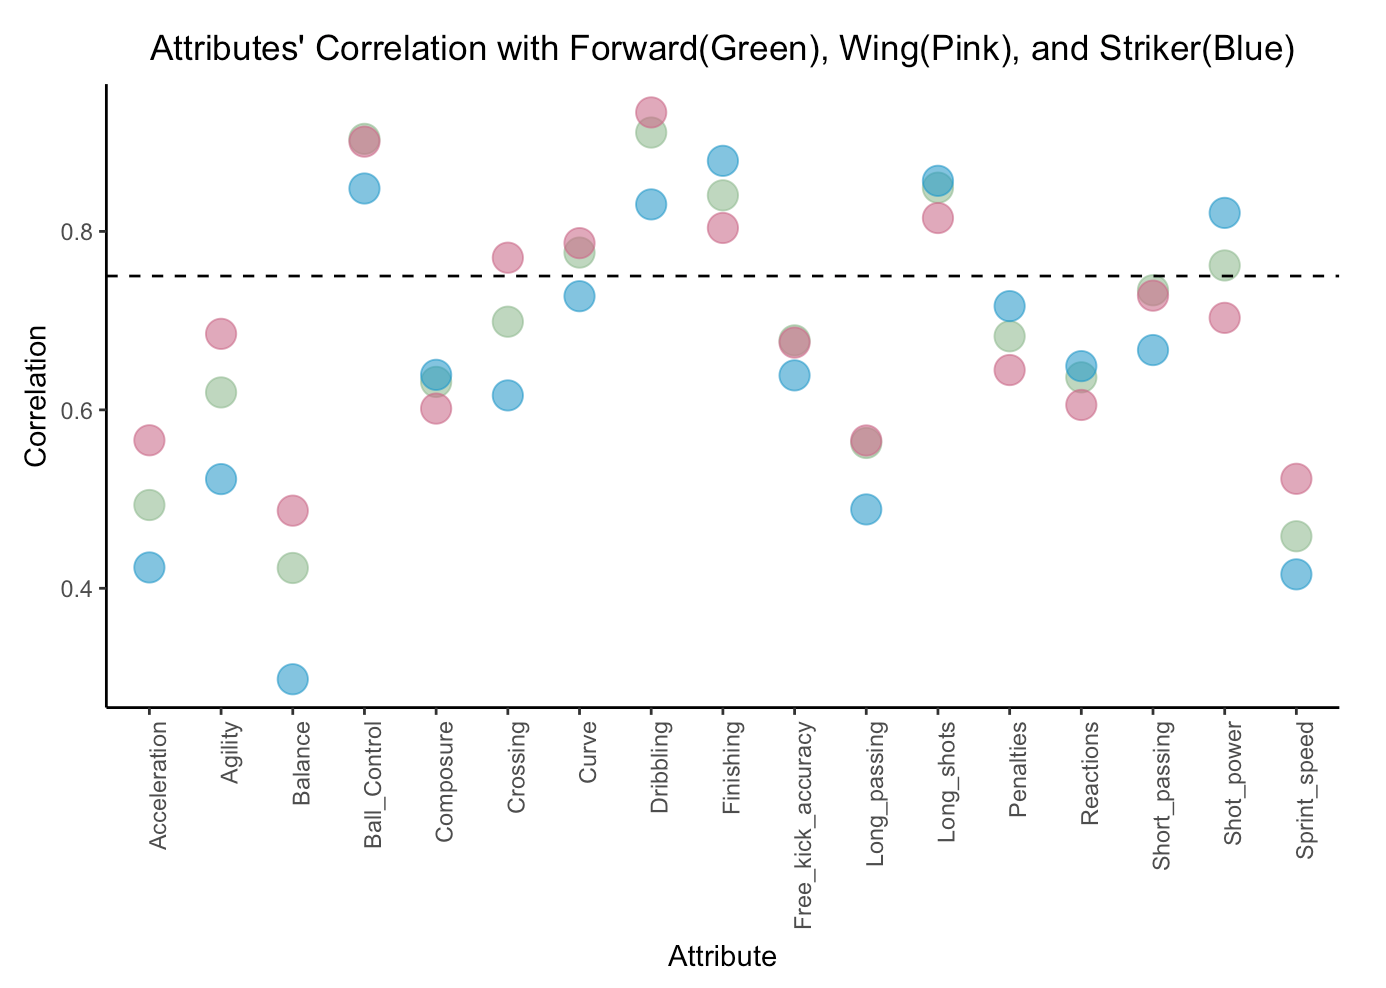
\includegraphics[width=1\linewidth]{images/corrplot2} The plot above
shows the same information in a slightly more intuitive way. The dashed
line is equal to a correlation value of 0.75 and is the baseline for
what my team and I decided should be classified as `important' to the
attacking position. The Attributes with the highest correlation to each
position score in a game represent which skills are more likely to be
linked with successful attackers in FIFA. The skills most associated
with an overall `Good Attacker': Ball Control, Dribbling, Finishing and
Long Shots.

\section{Carolina Data Challenge}\label{carolina-data-challenge}

\textbf{Context:}\\
In the fall of last year, my team and I competed in the first Carolina
Data Challenge and won a first prize award in the ``Best Insight''
category. Our entire collection of presentation material is on their
website here: \url{https://carolinadatachallenge.com/\#home}\\
In this competition, we were provided with data from Hurricane Harvey
Shelters detailing their reported needs. With the information provided,
we found that we could compile customized boxes for the shelters at a
lower cost than competing emergency boxes on the market, which often
didn't provide some basic needs required by each shelter. To convey the
needs generally, we created the visuals below.

\subsection{Word Cloud}\label{word-cloud}

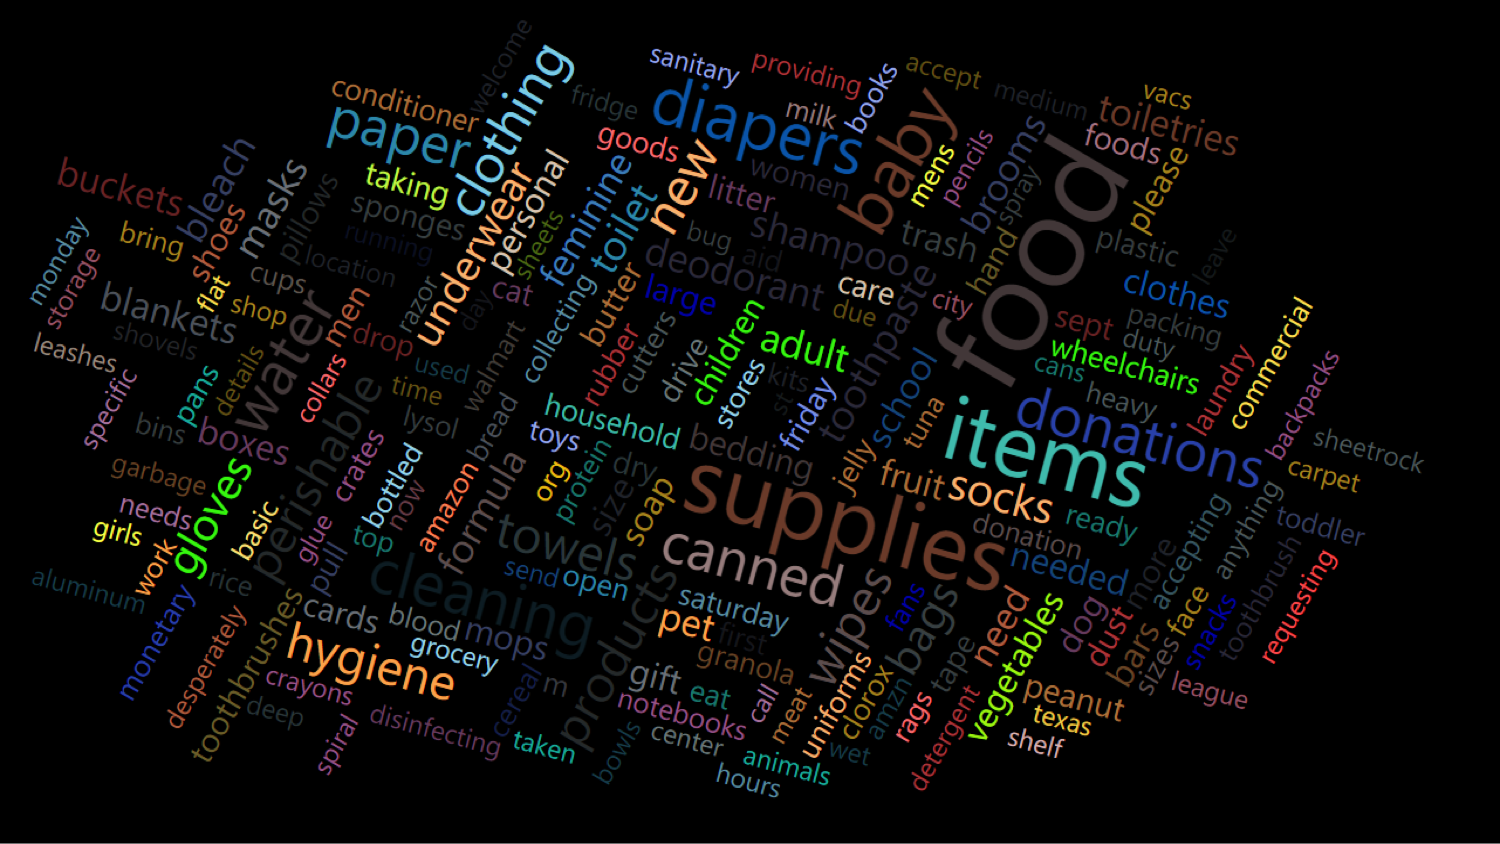
\includegraphics[width=1\linewidth]{images/wordcloud} The above visual
shows some of the most commonly requested items from shelters.

\subsection{Word Frequency Plot}\label{word-frequency-plot}

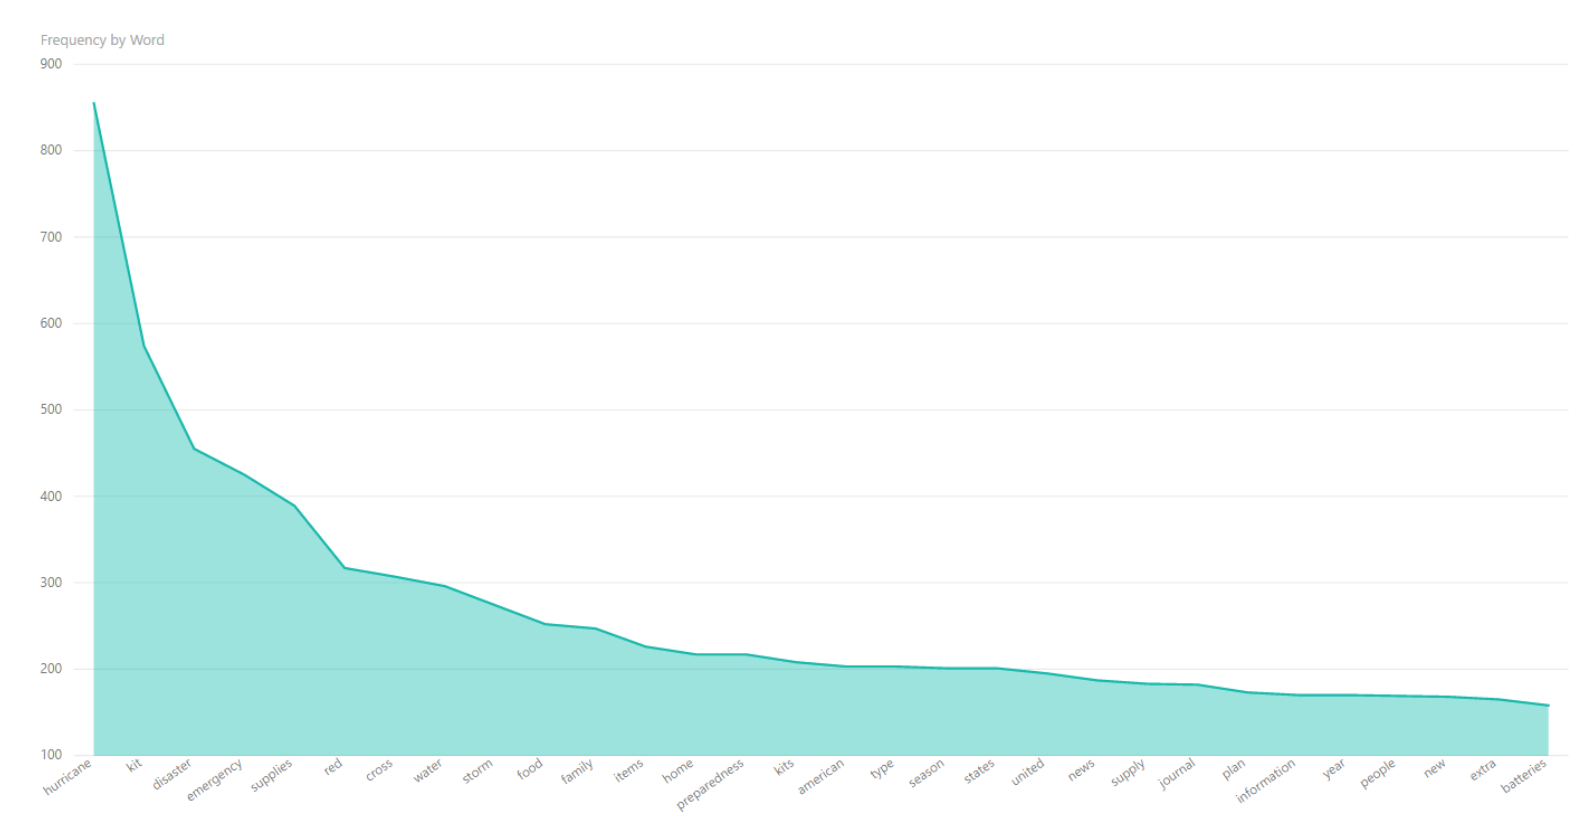
\includegraphics[width=1\linewidth]{images/wordfreq} The above shows our
frequency analysis of buckets of key words in the provided data along
with the first 100 articles found on the ProQuest Central database under
``Hurricane Emergency Kit''.


\end{document}
